\documentclass[urlcolor=blue,dvipsnames]{beamer}

\usepackage[utf8]{inputenc}
\usepackage{fancybox,fancyvrb}
\usepackage{environ,xspace,empheq}
\usepackage{tikz}
\hypersetup{colorlinks,linkcolor=,urlcolor=cyan}

\beamertemplatenavigationsymbolsempty
\setbeamertemplate{footline}[frame number]
\usetheme{Pittsburgh}

\newcommand\enumnum[1]{{\renewcommand{\insertenumlabel}{#1}%
      \usebeamertemplate{enumerate item} \,}}

\newcommand{\grad}{\nabla}
\newcommand{\ih}{\boldsymbol{\hat{\textbf{\i}}}}
\newcommand{\jh}{\boldsymbol{\hat{\textbf{\j}}}}
\newcommand{\vF}{\boldsymbol{\vec{\textbf{F}}}}
\newcommand{\Matlab}{\textsc{Matlab}\xspace}
\newcommand{\Octave}{\textsc{Octave}\xspace}


\title{9.1 Finding better numerical solutions \\ (than Euler's method)}

\subtitle{a lesson for MATH F302 Differential Equations}

\author{Ed Bueler, Dept.~of Mathematics and Statistics, UAF}

\date{\tiny \today}


\begin{document}
\setbeamertemplate{itemize item}{$\bullet$}
\setbeamertemplate{itemize subitem}{$\circ$}
\renewcommand{\thefootnote}{{\color{green} \arabic{footnote}}}

\begin{frame}
\titlepage

\centerline{\tiny for textbook: \, D. Zill, \emph{A First Course in Differential Equations with Modeling Applications}, 11th ed.}
%\color{green!40!blue}
\end{frame}


\begin{frame}{the situation}

these three facts make solving differential equations interesting:
\begin{enumerate}
\item DEs from science and engineering are usually \alert{not linear}
\item the by-hand methods which dominate Math 302\footnote{Chapters 2,4,6,7,8} are \alert{all weak}
    \begin{itemize}
    \item mostly they apply to linear DEs
    \item often they need the linear DE to have special coefficients
        \begin{itemize}
        \item ``special'' = constant, analytic, \dots
        \end{itemize}
    \end{itemize}
\item on the other hand, Euler's method is \alert{too inaccurate}
\begin{equation}
    y_{n+1} = y_n + h\, f(t_n,y_n)
\end{equation}

\vspace{-2mm}
    \begin{itemize}
    \item ``\emph{But whatever advantage {\normalfont (1)} has in its simplicity is lost in the crudeness of its approximations.}'' \hfill Zill, p.~369
    \item at least it does not care if your DE is linear or not
    \end{itemize}
\end{enumerate}
\end{frame}


\begin{frame}{but we can do better than Euler}

\begin{itemize}
\item here is the basic DE:
    $$\frac{dy}{dt} = f(t,y)$$

\vspace{-2mm}
    \begin{itemize}
    \item it could be a single equation or a system (\S4.10,5.3)
    \end{itemize}
\item at least numerical methods do not care if this DE is linear!
\item so we start again with Euler's method
    $$y_{n+1} = y_n + h\, f(t_n,y_n)$$
or equivalently
    $$\frac{y_{n+1} - y_n}{h} = f(t_n,y_n)$$
and \alert{try to do better}
\end{itemize}
\end{frame}


\begin{frame}{see slides and video on Euler's method}

\begin{itemize}
\item \alert{see my \S 2.6 slides and video}
    \begin{itemize}
    \item you must understand everything in those slides!
    \end{itemize}
\item they showed this sequence for $\frac{dy}{dt} = t - y^2$, $y(0)=1$:

\bigskip

\hspace{-12mm} \mbox{
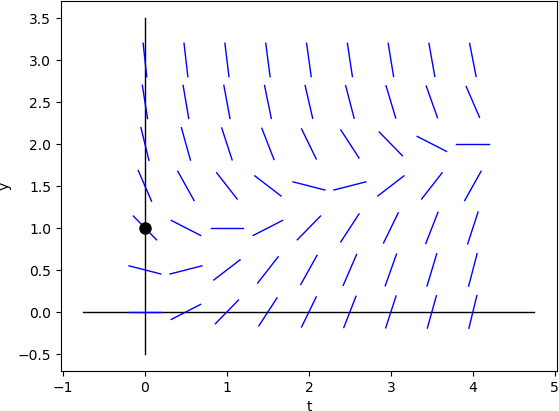
\includegraphics[width=0.31\textwidth]{figs/sequence-1} $\,$
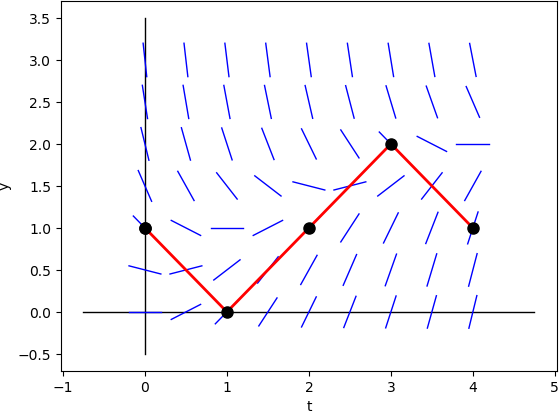
\includegraphics[width=0.31\textwidth]{figs/sequence-2} $\,$
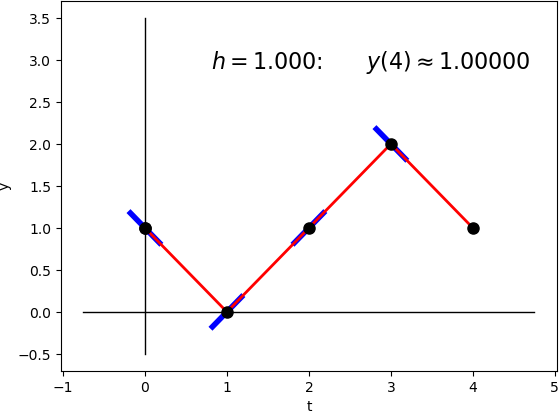
\includegraphics[width=0.31\textwidth]{figs/sequence-3} $\,$
}

\bigskip

\hspace{-12mm} \mbox{
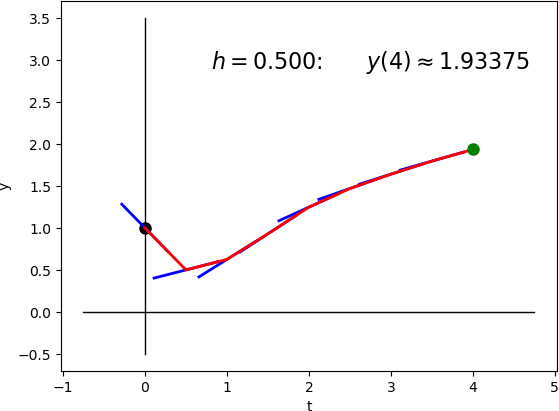
\includegraphics[width=0.31\textwidth]{figs/sequence-4} $\,$
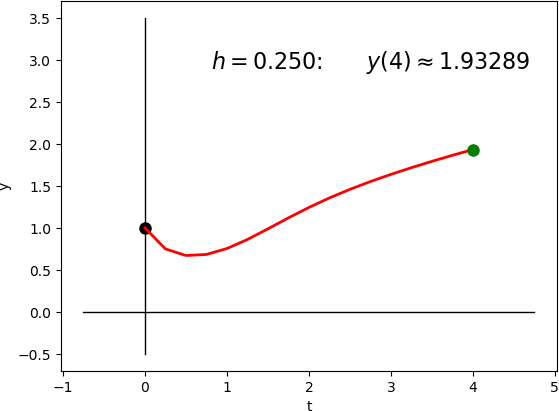
\includegraphics[width=0.31\textwidth]{figs/sequence-5} $\,$
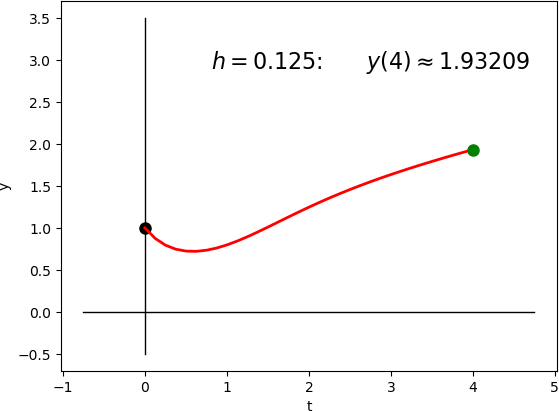
\includegraphics[width=0.31\textwidth]{figs/sequence-6}
}

    \begin{itemize}
    \item this visualization needs make sense! review Euler's method!
    \end{itemize}
\end{itemize}
\end{frame}


\begin{frame}[fragile]
\frametitle{Euler's method is a short code}

\bigskip
\VerbatimInput[fontsize=\footnotesize]{../codes/euler1.m}
\end{frame}


\begin{frame}[fragile]
\frametitle{example with \texttt{euler1.m}}

\begin{columns}
\begin{column}{0.55\textwidth}
\begin{itemize}
\item see comments:
\begin{Verbatim}[fontsize=\footnotesize]
>> help euler1
\end{Verbatim}
\item run the example:
\begin{Verbatim}[fontsize=\footnotesize]
>> f = @(t,y) t - y^2;
>> [tt,yy] = euler1(f,[0,4],1,0.5);
>> plot(tt,yy)
\end{Verbatim}
\item reduce step size and overlay:
\begin{Verbatim}[fontsize=\footnotesize]
>> [tt,yy] = euler1(f,[0,4],1,0.25);
>> hold on
>> plot(tt,yy,'r')
\end{Verbatim}
\end{itemize}
\end{column}
\begin{column}{0.45\textwidth}

\mbox{\quad 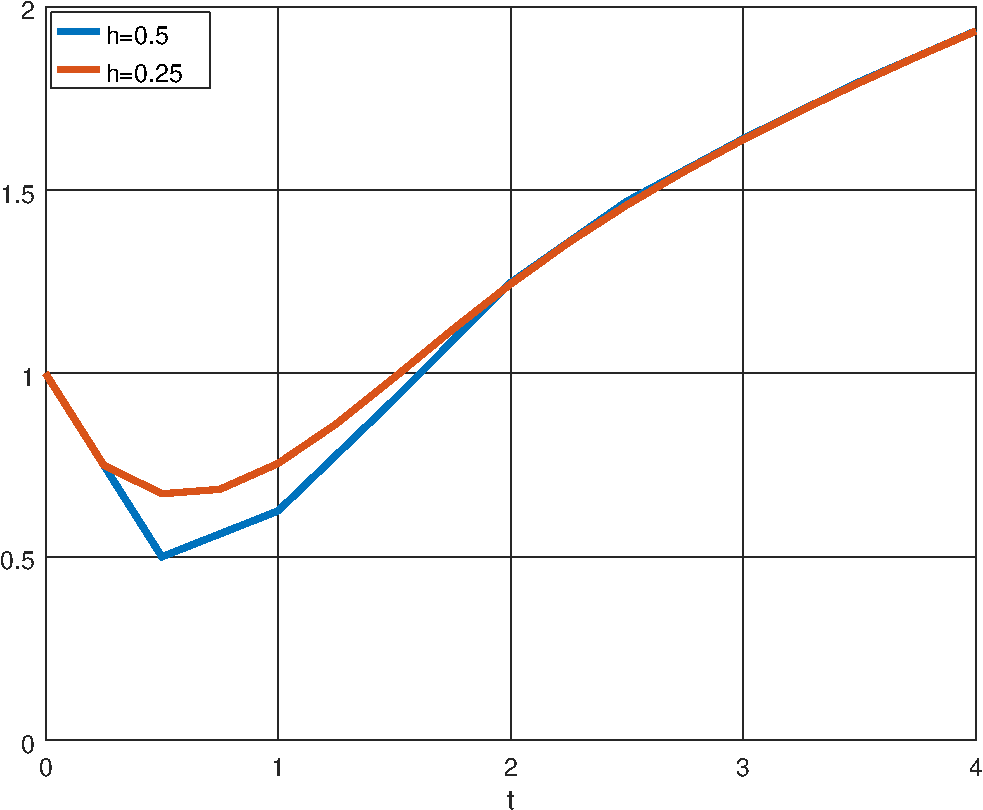
\includegraphics[width=\textwidth]{figs/euler1basic}}
\end{column}
\end{columns}
\end{frame}


\begin{frame}[fragile]
\frametitle{from Euler to \texttt{ode45} in three steps}

\begin{itemize}
\item use of \texttt{euler1} should look familiar
\item it is just like how we used \texttt{ode45} in \S5.3 and \S4.10
\item notice the first line of the code:
\end{itemize}
\end{frame}


\begin{frame}{x}

\begin{itemize}
\item X
\end{itemize}
\end{frame}

% for problem:
% >> f = @(t,y) t - y^2;
% >> optt = odeset('RelTol',RTOL,'AbsTol',1.0e-14);
% >> [tt,yy] = ode45(f,[0,4],1,optt); yy(end)
%ans =  1.93122683184240
%       -----------       <- 10 digits which agree for
%                            RTOL=1.0e-9,1.0e-10,1.0e-11,1.0e-12

% will use:  yexact = 1.9312268318427   based on above and RK4 with h=0.0001

% on same problem, for considering refinement:
% h=0.4, 0.2, 0.1, 0.05, 0.025

\begin{frame}{expectations}

\begin{itemize}
\item just watching this video is \emph{not} enough!
     \begin{itemize}
     \item see ``found online'' videos and stuff at

     \centerline{\href{https://bueler.github.io/math302/week10.html}{\tt \color{cyan} bueler.github.io/math302/week10.html}}
     \item \emph{read} section 9.1 in the textbook
     \item \emph{do} the WebAssign exercises for section 9.1
     \end{itemize}
\end{itemize}
\end{frame}

\end{document}

